\documentclass[a4paper]{article}
\usepackage[T1]{fontenc}
\usepackage[utf8]{inputenc}
\usepackage{lmodern}
\usepackage[polish]{babel}
\usepackage{amsfonts}
\usepackage{graphicx}
\usepackage{hyperref} 

\title{Dokumentacja \\ Problem Komiwojażera \\ na NetBeans Platform}
\author{Bartek Bułat \\ Konrad Malawski \\ Michał Nowak}
\date{08.06.2010}

\pdfinfo{
  /Title    (Dokumentacja --- Problem Komiwojażera - na NetBeans Platform)
  /Author   (Bartek Bułat Konrad Malawski, Michał Nowak)
  /Creator  (Konrad Malawski)
  /Keywords (NetBeans Platform, Traveling Salesman)
}

\begin{document}
\maketitle
\newpage

\tableofcontents
\newpage

%%%%%%%%%%%%%%%%%%%%%%%%%%%%%%%%%%%%%%%%%%%%%%%%%%%%%%%%%%%%%%%%%%%%%%%%%%%%%%%%%%%%%%%%%%%%%
\section{Problem komiwojażera}
Zagadnieniem naszego projektu był jeden z najstarszych problemów związanych z teorią grafów – problem komiwojażera (Traveling Salesman Problem). Tematem tego zagadnienia patrząc od strony teorii grafów jest znalezienie minimalnego cyklu Hamiltona w k-klice, gdzie podane są wagi wszystkich krawędzi. Problem ten obrazowany jest z punktu widzenia komiwojażera (akwizytora) który chce odwiedzić wszystkie miasta, przy czym w każdym chce być dokładnie raz i nie chce dwa razy chodzić tą samą drogą. Zna on odległości pomiędzy każdymi dwoma miastami i wszystkie miasta są ze sobą połączone. Istnieje bardziej skomplikowana wersja tego problemu – wersja asymetryczna. Problem tamten różni się tym, że droga z pierwszego do miasta drugiego może mieć inną długość, niż droga powrotna. W naszym projekcie skupiliśmy się jednak na bardziej popularnej i standardowej wersji tego problemu grafowego.

\subsection{Problem komiwojażera jako NP-zupełny}
Zagadnienie związane z naszym projektem w teorii grafów, przy podejściu decyzyjnym uznane jest za należące do klasy NP-zupełnych. Należenie do klasy NP oznacza, że w czasie wielomianowym, możliwe jest sprawdzenie czy podane rozwiązanie jest poprawne. Ale samo rozwiązanie problemu nie jest możliwe. Definicja klasy NP-zupełnej jest bardziej skomplikowana. Dowód należenia problemu komiwojażera do tej klasy można znaleźć w [1] na stronie 1036. Przykładem problemu klasy NP jest problem znalezienia cyklu Hamiltona (w skończonym czasie jesteśmy w stanie sprawdzić, czy podana sekwencja wierzchołków tworzy cykl), problem komiwojażera rozszerza to zagadnienie (po otrzymaniu sekwencji węzłów możemy policzyć koszt przebycia trasy, ale nie mamy pewności, że jest ona najkrótszą z możliwych). Dlatego nasz problem jest „tak trudny jak dowolny problem w NP” [1] (strona 991).

\subsection{Podejście algorytmiczne, a heurystyczne}
Podejście algorytmiczne do problemu komiwojażera, gwarantuje rozwiązanie optymalne. Ilość przypadków do rozpatrzenia przy n wierzchołków wynosi n! Więc sprawdzanie wszystkich możliwych rozwiązań może być skuteczne tylko dla bardzo małych ilości węzłów. Przy większej ilości węzłów czas oczekiwania na wynik ostateczny zmierza do nieskończoności, a dodanie każdego kolejnego węzła (numer n+1) tylko zwiększa ten czas (ilość przypadków do rozważenia rośnie n+1 – krotnie).  Podejściem całkiem odmiennym jest heurystyczne spojrzenie na ten problem. Trzeba być jednak świadomym wad tego rozwiązania. To podejście nie daje nam gwarancji znalezienia najlepszego rozwiązania, ale daje gwarancje obliczeń w skończonym czasie i zakończenie ich w jakimś minimum lokalnym (być może ekstremum globalnym). Lecz podejście drugie ze względu na gwarancję otrzymania wyniku zostało wykorzystane w tym projekcie. W celu implementacji tego podejścia wykorzystane są algorytmy genetyczne.

%%%%%%%%%%%%%%%%%%%%%%%%%%%%%%%%%%%%%%%%%%%%%%%%%%%%%%%%%%%%%%%%%%%%%%%%%%%%%%%%%%%%%%%%%%%%%
\section{Rozwiązanie problemu komiwojażera przy użyciu algorytmów ewolucyjnych}
Mamy zamiar teraz przedstawić nasz sposób rozwiązania tego NP-zupełnego problemu wykorzystując algorytmy decyzyjne. W kolejnych punktach opisze struktury oraz mechanizmy stworzone i wykorzystane przez nas na potrzeby projektu. Zawierają się w nich: struktura chromosomu, losowanie populacji początkowej, kryterium oceny osobników, metody selekcji (używane przez nas: metoda ruletki i metoda turniejowa), proces krzyżowania (krzyżowanie OX oraz heurystyczne), a także wykorzystany przez nas sposób mutowania osobników.

\subsection{Chromosomy}
Spośród trzech możliwych reprezentacji (ścieżkowej, przyległościowej i porządkowej) chromosomu możliwych do wykorzystania w naszym projekcie wybraliśmy reprezentacje ścieżkową. Reprezentacja chromosomu zawiera u nas ciąg wartości odpowiadających kolejnym węzłom (miastom) cyklu. Reprezentacja ta jest najbliższa i najbardziej przejrzysta dla ludzi. Lecz jej wadą jest trudność w implementacji krzyżowania. Chromosomy można tworzyć z wykorzystaniem algorytmu zachłannego. Wersja bez algorytmu zachłannego przypisuje kolejnym wartością losowe numery węzłów w grafie. Wersja zachłanna różni się tym, że trasa jest już w procesie tworzenia optymalizowana. Wybierany jest pierwszy węzeł, a następnie wybierany jest kolejny położony najbliżej i tak zapełniany jest cały chromosom.

\subsection{Losowanie populacji początkowej}
Odbywa się na podstawie wprowadzonej zmiennej (liczba osobników populacji), generowana jest wybrana ilość chromosomów w sposób opisany powyżej (możliwa opcja zachłanna).

\subsection{Kryterium oceny osobników}
Kryterium w przypadku naszego projektu jest po prostu długość ścieżki (cyklu), dążymy do jak najmniejszej wartości tego parametru, a więc kryterium przystosowania w naszym przypadku jest odwrotnie proporcjonalne do wartości długości cyklu.

\subsection{Metody selekcji}
W naszym projekcie w celu wprowadzenie zróżnicowania i możliwości porównania skuteczności postanowiliśmy wdrożyć dwie metody selekcji: poprzez ruletkę oraz metodę turniejową.

\textbf{Metoda ruletki} --- polega na wielokrotnym (dokładnie tyle ile mamy osobników) losowaniu osobników z pierwotnej populacji. Osobniki te przepisane zostaną do nowej populacji. Losowanie odbywa się poprzez stworzenie „koła fortuny” w którym osobniki lepsze (o większym kryterium przystosowania), zajmują większy obszar. Dzięki temu zabiegowi mają one większe prawdopodobieństwo na przeniesienie do kolejnego pokolenia. Wadą tego rozwiązania jest, stosunkowo szybkie zbieganie się do ewentualnego minimum lokalnego.

\textbf{Metoda turniejowa} --- druga wybrana przez nas metoda, ma całkiem inne parametry, niż ruletka. Jest ona bardziej odporna na zbieganie się do minimum lokalnych. Jest tak dlatego, że przy każdym z n losowań, wybierana jest podgrupa osobników z których do kolejnego pokolenia przechodzi tylko najlepiej dopasowany. Ta zwiększona losowość chroni przed zbyt szybkim zbieganiem się. Zastosowany u nas sposób jest uproszczoną metodą turniejową. Przeprowadzany jest turniej wśród wszystkich osobników, w którym wygrywa lepsza połowa (sortujemy rosnąco wszystkie osobniki i wybieramy połowę lepiej przystosowaną), którą krzyżujemy z losowym osobnikiem z gorszej połowy, dzięki czemu dłużej zachowana jest różnorodność. Powstaje w ten sposób nowe pokolenie które przechodzi do następnego cyklu.

\subsection{Proces krzyżowania}
W procesie tworzenia grafu w naszym projekcie możliwy jest wybór typu krzyżowania. Dostępne jest krzyżowanie OX (popularne) oraz krzyżowanie heurystyczne (w tym przypadku na decyzje mają wpływ obecne warunki zadania). Poszczególne metody przedstawiają się następująco:

\textbf{Metoda OX }polega na przeniesieniu pewnej losowej części z jednego chromosomu-rodzica i uzupełnieniu wartościami z drugiego, przy zachowaniu kolejności ich występowania i poczynając od tylniej części chromosomu-dziecka. Ogólnie metoda ta polega na wymianie pewnej środkowej części genotypu i uzupełnieniu wartościami drugiego niezmienionego chromosomu, w ramach możliwości. W trakcie prac nad projektem udało nam się zauważyć, że metoda OX nie gwarantuje dobrej zbieżności, co skłoniło nas do implementacji innej metody.

\textbf{Metoda heurystyczna} w naszym projekcie działa następująco. Dane są dwa chromosomy - rodzice z których będą wybierane lepsze warianty. Kolejnym krokiem jest losowanie dowolnego węzła. Kolejnym krokiem jest sprawdzenie w którym chromosomie – rodzicu kolejne miasto leży najbliżej, a następnie wybranie i przepisanie go. Jeżeli nie jest to możliwe następuje wybór możliwości z drugiego rodzica. Jeżeli obydwa węzły zostały  już wykorzystane w potomku, następuje przepisanie kolejnego najbliższego wariantu. W momencie wywoływania tego krzyżowania jest on wywoływane dla każdego z chromosomów pełniących rolę z rodzica, z parametrem w postaci drugiego z tych osobników. Zachowanie takie ma na celu stworzenie dwójki potomnych dzieci.

\subsection{Mutowanie}
Proces ten w naszym projekcie oparliśmy na prostym wylosowaniu dwóch różnych węzłów na drodze komiwojażera i zamienieniu ich miejscami. Procesowi mutacji podlega co cykl ilość osobników równa: (ilość pokoleń bez poprawy)/(max ilość pokoleń bez poprawy)*0.5 (oba parametry można ustawić w momencie tworzenia grafu).

\subsection{Warunek stopu}
W celu zakończenia naszego algorytmu stworzyliśmy dwa warunki stopu, zależne od dwóch zmiennych wprowadzanych przez użytkownika. Ilość pokoleń bez poprawy – jeżeli przez zadaną liczbę pokoleń najlepszy osobnik w nie będzie ulegał zmianą, algorytm zatrzyma się, ponieważ poprawienie wynik jest już prawdopodobnie niemożliwe. Drugim warunkiem stopu jest maksymalna ilość pokoleń, po przekroczeniu zadanej wartości algorytm zatrzyma się, ze względu na wystarczająco długi czas jego trwania, lub z powodu takich ustawień wprowadzonych przez użytkownika. Oczywiście można też wymusić zatrzymanie algorytmu poprzez dostępne w interfejsie użytkownika opcje.

%%%%%%%%%%%%%%%%%%%%%%%%%%%%%%%%%%%%%%%%%%%%%%%%%%%%%%%%%%%%%%%%%%%%%%%%%%%%%%%%%%%%%%%%%%%%%
\section{Parametry programu}
\begin{figure}[phb]
 \centering
 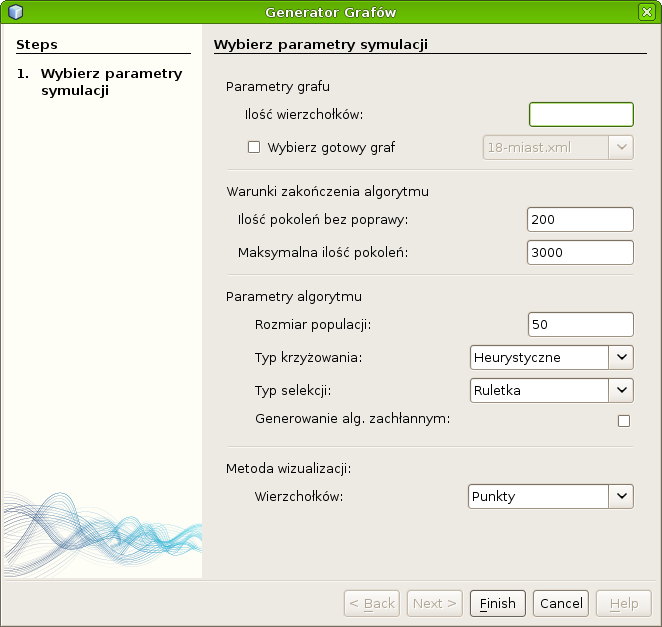
\includegraphics[width=\textwidth ]{wizard.png}
 \caption{Generator grafów}
\end{figure}

Na załączonym rysunku widać okno które pozwala nam wygenerować graf w którym będziemy szukać minimalnego cyklu. Nasz projekt udostępnia użytkownikowi takie opcje jak:
Ilość wierzchołków – w zależności od wartości tego parametru, generowany jest graf pełny o zadanej liczbie węzłów.
Wybierz gotowy graf – na potrzeby projektu stworzone zostało kilkanaście grafów, na których można bardzo przejrzyście zaobserwować proces wyznaczania minimalnego cyklu. Niektóre grafy, mają też swoje odwzorowanie na mapach Polski i liczą cykle dla wybranych miast.
Ilość pokoleń bez poprawy – parametr ten jest pierwszym warunkiem stopu, określa on, ile razy pod rząd może nie wystąpić zmiana u najlepszego osobnika populacji, jeżeli wartość ta zostanie osiągnięta program zakończy działanie.

\begin{itemize}
 \item \textbf{Maksymalna ilość pokoleń} --- drugi warunek stopu, po osiągnięciu tej wartości podczas procesów krzyżowania program zostanie zatrzymany. Pokolenie o indeksie równym temu parametrowi będzie ostatnim potomstwem.

 \item \textbf{Rozmiar populacji} --- określa ilość chromosomów zawierających się w każdej populacji, zwiększenie tej wartości powoduje zwiększenie szans na znalezienie ekstremum globalnego, ale jest to osiągane kosztem czasu (zwiększa się ilość obliczeń, a co za tym idzie ich czas). Zmniejszenie go, zwiększa szanse na to, że nasze obliczenia zatrzymają się na pewnym minimum lokalnym, ale przyśpiesza działanie programu.

 \item \textbf{Typ krzyżowania} --- przełącza pomiędzy zaimplementowanymi przez nas rodzajami krzyżowania. W programie dostępne są krzyżowania typu OX oraz krzyżowanie heurystyczne. Opis różnic poszczególnych krzyżowań zawiera się w części 2.d.

 \item \textbf{Typ selekcji} --- podobnie jak parametr wyżej, ustawia jeden z dostępnych rodzajów selekcji. W projekcie zaimplementowane zostały selekcje metodą ruletki oraz uproszczoną metodą turniejową. Opisy tych metod znaleźć można w sekcji 2.e.

 \item \textbf{Gen. alg. zachłannym} --- zaznaczenie tej opcji spowoduje wykorzystanie algorytmu zachłannego w procesie tworzenia chromosomów (w trakcie generowania populacji początkowej). Spowoduje to jeszcze szybsze zbieganie się algorytmu. Opis tego algorytmu znajduje się w podpunkcie 2.a.

 \item \textbf{Metoda wizualizacji wierzchołków} --- do wyboru mamy tutaj dwie opcje. Wybór punktów polecany jest szczególnie przy większych grafach, a także dla zwiększenia przejrzystości grafu. Opcja z etykietami miast jest dużo ciekawsza, jeżeli obserwujemy działanie algorytmu na przykładzie grafu który odwzorowuje położenie geograficzne określonych miast i na ich przykładzie rozwiązuje problem komiwojażera.
\end{itemize}


%%%%%%%%%%%%%%%%%%%%%%%%%%%%%%%%%%%%%%%%%%%%%%%%%%%%%%%%%%%%%%%%%%%%%%%%%%%%%%%%%%%%%%%%%%%%%
\section{Wykorzystane technologie/frameworki}
Projekt został stworzony przy wykorzystaniu tylko i wyłącznie wolnego oprogramowania jak i korzysta z wolnych bibliotek oraz frameworków. Poniżej kilka słów o najważniejszych z nich, celem przybliżenia dlaczego zostały wybrane, i czy polecilibyśmy je do wykorzystania innym.

\subsection{NetBeans Platform}
Projekt został napisany w Javie, korzystając z NetBeans Platform (w wersji 6.8). Przed rozpoczęciem programowania naszej aplikacji wszyscy uczestniczyliśmy w szkoleniu \textit{NetBeans Platform Certified Training} które organizował Konrad jako członek \textit{Polish Java User Group}. Więcej informacji o samym szkoleniu można znaleźć pod: \href{http://www.netbeans.edu.pl}{netbeans.edu.pl}.

Powodem wyboru NBP jako platformy do rozwoju naszej aplikacji były ogólne zalety frameworków, czyli przyśpieszonego cyklu rozwoju samej aplikacji oraz konkretne zalety NetBeans Platform tj. budowa \textit{modularnych aplikacji}. Realne aplikacje generalnie nie są już obecnie pisane nie-modularnie, powodem są oczywiste zalety płynące z luźnego wiązania aplikacji, czyli możliwość niezależnej pracy nad poszczególnymi modułami przez programistów - nie przeszkadzając sobie zmianami ew. udostępnianych metod. 

Do realizacji luźnego wiązania między modułami - konkretniej między 'algorytmem' oraz 'elementami 'rysującymi graf wynikowy' został wykorzystany wzorzec Observer/Observable zaimplementowany przy wykorzystaniu Lookup'ów (jednej z zalet NetBeans Platform). Implementację tą Konrad przedstawił na dZone.com za prośbą Pana Wielenga (Technical Writer w Sun Microsystems) do publikacji tegoż tekstu tam: \href{http://netbeans.dzone.com/articles/netbeans-platform-lookups}{NetBeans Platform Lookups as Communication Method}.

Bardzo ważną zaletą NetBeans Platform, odróżniającą ją na przykład od \textit{Eclipse RCP} lub \textit{Spring RCP} jest bazowanie na Swing - dzięki czemu nie występują problemy podczas integracji istniejących rozwiązań (prefuse, jfreechart etc) z aplikacją bazującą na NetBeans RCP - co w przypadku Eclipse RCP potencjalnie mogłoby sprawić duże problemy, jako że bazuje on na SWT (natywnych kontrolkach).

\subsection{Prefuse}
Prefuse jest dostępną pod \href{http://prefuse.org/}{http://prefuse.org/} wolnoźródłową biblioteką implementującą różne wizualizacje oraz reprezentacje grafów. Niestety projekt jest od lat martwy i nigdy nie osiągnął wersji stabilnej. Dokumentacja również jest bardzo nie pełna, i pozostaje korzystanie z samego JavaDoc, co do naszych celów jednak jak najbardziej wystarczało. 

Cykl rysowania grafu w prefuse idealnie wpasował się w nasz problem do rozwiązania. Deklaruje się pewne 'akcje', które następnie są wołane w pewnych odstępach czasu, dokładnie tak jest wołany nasz algorytm rozwiązywania problemu komiwojażera. Warto nadmienić iż listy akcji mogą być od siebie niezależne i dzięki temu rysowanie/kolorowanie grafu nie musi blokować liczenia algorytmu. 

Inną zaletą jest wbudowana obsługa parsowania GraphML --- była ona de facto głównym czynnikiem wyboru tej biblioteki.

\subsection{GraphML}
Program korzysta z plików XML zapisywanych w folderze data w celu przechowywania danych o wygenerowanych (oraz dostępnych predefiniowanych) grafach. Format tych plików jest ściśle określony przez \href{http://graphml.graphdrawing.org/specification.html}{specyfikację GraphML}, dzięki czemu możliwe jest sprawdzenie naszych algorytmów na dowolnym grafie - dostarczonym do folderu data w postaci pliku zgodnego z GraphML.

\subsection{JFreeChart}
Do rysowania wykresów zbieżności algorytmu użyliśmy bardzo dobrej biblioteki jaką jest JFreeChart. Jest ona dostępna na licencji LGPL pod następującym adresem: \href{http://www.jfree.org/jfreechart/}{http://www.jfree.org/jfreechart/}. Biblioteka ta jest dość znana stąd pominę głębsze rozważania nad jej przydatnością --- słowem: jest najlepszą (wolnoźródłową) znaną nam biblioteką służącą do wizuzalizacji wykresów.

\section{Kod źródłowy oraz licencja}
Kod źródłowy programu był rozwijany od początku do końca pod kontrolą systemu kontroli wersji \textbf{Git} a repozytorium znajduje się pod:

\begin{flushleft}
\href{http://github.com/ktoso/TravelingSalesman-NBP}{http://github.com/ktoso/TravelingSalesman-NBP}                                                                                                   \end{flushleft}

Możliwe do wglądu są kolejne 'wydania' (tagi) jak i najświeższa wersja kodu. Program będzie w całości licencjonowany na warunkach \textbf{GPLv3} --- odpowiednie adnotacje w kodzie źródłowym zostaną dodane już niebawem.

\end{document}
